\documentclass[12pt,a4paper]{article}

\usepackage[T1]{fontenc}
\usepackage[utf8]{inputenc}
\usepackage[margin=2.5cm,headheight=15pt]{geometry}
\usepackage{graphicx}
\usepackage{float}
\usepackage{xcolor}
\usepackage{listings}
\usepackage{fancyhdr}
\usepackage{hyperref}

\graphicspath{{images/}}
\pagestyle{fancy}
\fancyhf{}
\fancyhead[L]{Lab 03 -- Buttons/Switches}
\fancyhead[R]{MPU \& MCU}
\fancyfoot[C]{\thepage}
\renewcommand{\headrulewidth}{0.4pt}
\renewcommand{\footrulewidth}{0pt}

\lstset{
    language=C,
    basicstyle=\ttfamily\footnotesize,
    keywordstyle=\color{blue},
    commentstyle=\color{gray},
    stringstyle=\color{red},
    numbers=left,
    numberstyle=\tiny\color{gray},
    numbersep=6pt,
    frame=single,
    breaklines=true,
    keepspaces=true,
    columns=fullflexible,
    showstringspaces=false,
    tabsize=4,
    captionpos=b
}

\begin{document}

\section{Exercise 1}

\begin{figure}[H]
    \centering
    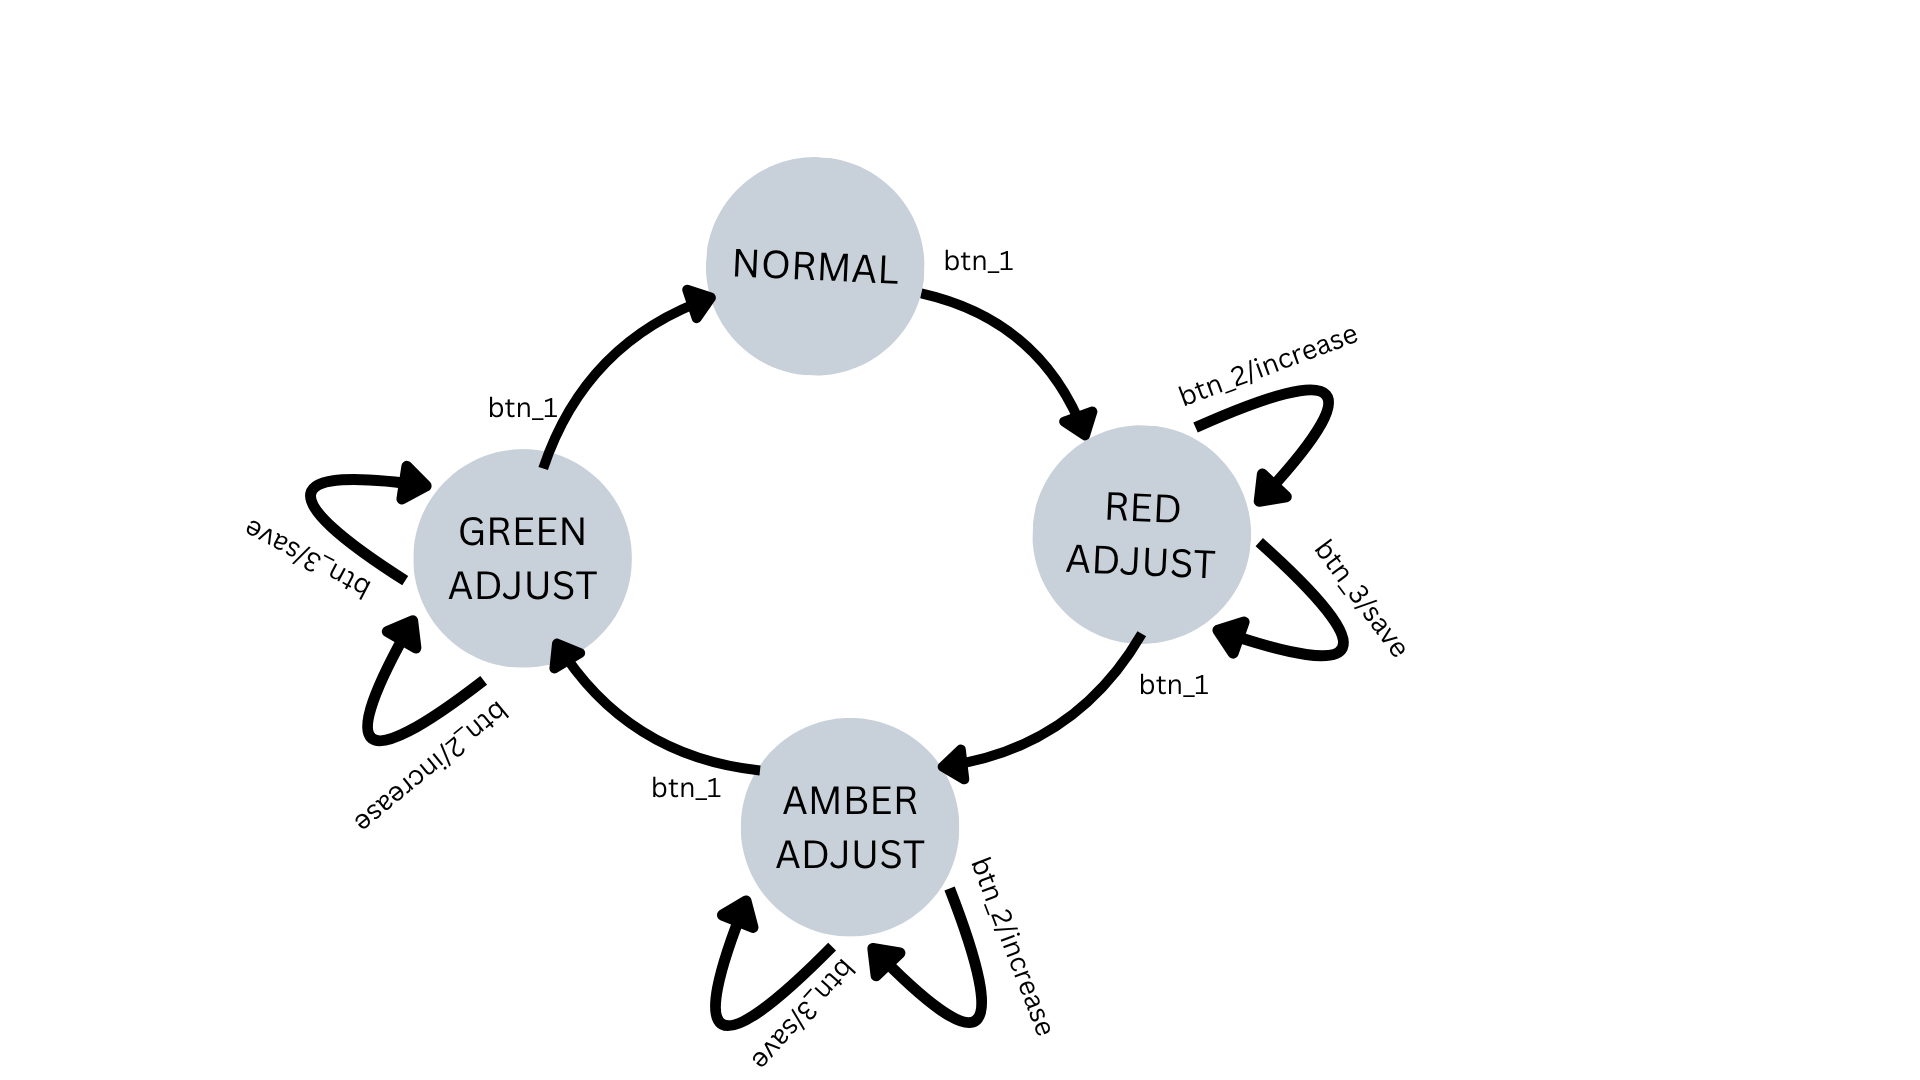
\includegraphics[width=\textwidth,height=0.65\textheight,keepaspectratio]{exercise_1_fsm.png}
    \caption{Finite state machine -- Exercise 1}
    \label{fig:fsm}
\end{figure}

The system has four modes: normal operation, red adjustment, amber adjustment,
and green adjustment. BTN1 cycles through these modes. In an adjustment mode,
BTN2 increases the temporary duration and BTN3 saves it without leaving the mode.
The saved duration is used when normal operation is restarted.

\section{Exercise 2}

\begin{figure}[H]
    \centering
    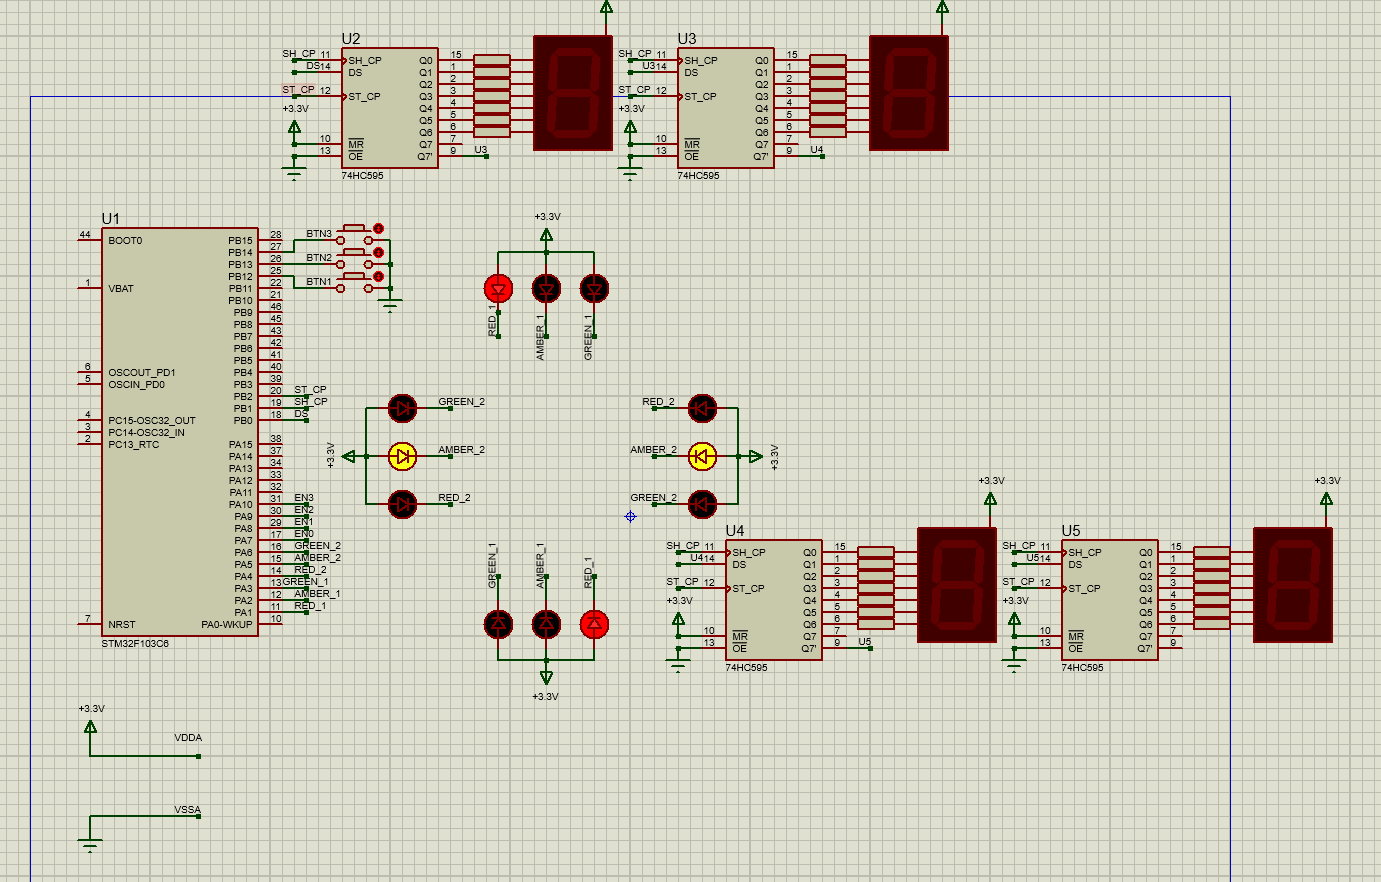
\includegraphics[width=\textwidth,height=0.65\textheight,keepaspectratio]{exercise_2_74hc595.png}
    \caption{Proteus schematic with four 74HC595 registers -- Exercise 2}
    \label{fig:schematic}
\end{figure}

The circuit uses an STM32F103C6, twelve traffic LEDs, four common-anode
seven-segment displays, and three active-low buttons. Opposite traffic lights
share the same control signals.

Each seven-segment display is driven by one 74HC595. The registers are connected
in the order U2, U3, U4, and U5. Q0--Q6 connect to segments a--g through separate
1 k$\Omega$ resistors. Q7 is unused. The common anodes connect to 3.3 V.
The serial output Q7$'$ of each register connects to DS of the next register.
SH\_CP and ST\_CP are shared by all four registers.

MR is connected to 3.3 V and OE to ground. The hidden VCC/GND pins must be
powered, with the VCC/VDD rail set to 3.3 V. The original Proteus display model
uses a Segment On Current of 1 mA. Each register holds its output between updates,
so the four digits remain visible without multiplex scanning.

\section{Exercise 3}

The GPIO configuration follows the final schematic. The traffic LEDs are
active-low outputs. The three buttons use internal pull-ups and connect to
ground when pressed.

\begin{center}
\begin{tabular}{lll}
\hline
Signal & MCU pin & Function \\
\hline
RED\_1, AMBER\_1, GREEN\_1 & PA1--PA3 & Road 1 lights \\
RED\_2, AMBER\_2, GREEN\_2 & PA4--PA6 & Road 2 lights \\
DS & PB0 & Serial data to U2 \\
SH\_CP & PB1 & Shift clock \\
ST\_CP & PB2 & Output latch clock \\
BTN1, BTN2, BTN3 & PB12--PB14 & Mode, increase, save \\
\hline
\end{tabular}
\end{center}

TIM2 is configured for a 10 ms interrupt using the 8 MHz internal clock:
\[
T=\frac{(7999+1)(9+1)}{8\,000\,000}=0.01\ \mathrm{s}.
\]

\noindent\begin{minipage}{\linewidth}
\begin{lstlisting}[caption={GPIO initialization -- Exercise 3}]
static void MX_GPIO_Init(void)
{
  GPIO_InitTypeDef GPIO_InitStruct = {0};

  __HAL_RCC_AFIO_CLK_ENABLE();
  __HAL_AFIO_REMAP_SWJ_NOJTAG();

  __HAL_RCC_GPIOA_CLK_ENABLE();
  __HAL_RCC_GPIOB_CLK_ENABLE();

  HAL_GPIO_WritePin(GPIOA, RED_1_Pin | AMBER_1_Pin | GREEN_1_Pin |
                           RED_2_Pin | AMBER_2_Pin | GREEN_2_Pin,
                           GPIO_PIN_SET);
  HAL_GPIO_WritePin(GPIOB, DISPLAY_DATA_Pin | DISPLAY_CLOCK_Pin | DISPLAY_LATCH_Pin,
                           GPIO_PIN_RESET);

  GPIO_InitStruct.Pin = RED_1_Pin | AMBER_1_Pin | GREEN_1_Pin |
                        RED_2_Pin | AMBER_2_Pin | GREEN_2_Pin;
  GPIO_InitStruct.Mode = GPIO_MODE_OUTPUT_PP;
  GPIO_InitStruct.Pull = GPIO_NOPULL;
  GPIO_InitStruct.Speed = GPIO_SPEED_FREQ_LOW;
  HAL_GPIO_Init(GPIOA, &GPIO_InitStruct);

  GPIO_InitStruct.Pin = DISPLAY_DATA_Pin | DISPLAY_CLOCK_Pin | DISPLAY_LATCH_Pin;
  GPIO_InitStruct.Mode = GPIO_MODE_OUTPUT_PP;
  GPIO_InitStruct.Pull = GPIO_NOPULL;
  GPIO_InitStruct.Speed = GPIO_SPEED_FREQ_LOW;
  HAL_GPIO_Init(GPIOB, &GPIO_InitStruct);

  GPIO_InitStruct.Pin = BTN1_Pin | BTN2_Pin | BTN3_Pin;
  GPIO_InitStruct.Mode = GPIO_MODE_INPUT;
  GPIO_InitStruct.Pull = GPIO_PULLUP;
  HAL_GPIO_Init(GPIOB, &GPIO_InitStruct);
}
\end{lstlisting}
\end{minipage}

\noindent\begin{minipage}{\linewidth}
\begin{lstlisting}[caption={TIM2 configuration excerpt -- Exercise 3}]
htim2.Instance = TIM2;
htim2.Init.Prescaler = 7999;
htim2.Init.CounterMode = TIM_COUNTERMODE_UP;
htim2.Init.Period = 9;
htim2.Init.ClockDivision = TIM_CLOCKDIVISION_DIV1;
htim2.Init.AutoReloadPreload = TIM_AUTORELOAD_PRELOAD_DISABLE;
HAL_TIM_Base_Init(&htim2);
HAL_TIM_Base_Start_IT(&htim2);
\end{lstlisting}
\end{minipage}

\section{Exercise 4}

Timing is expressed in milliseconds using \texttt{HAL\_GetTick()}, which is
updated by the 1 ms SysTick interrupt. It is independent of the TIM2 period.
With the prescaler fixed at 7999, changing TIM2's period from 9 to 0 or 99
selects a 1 ms or 100 ms interrupt. The application deadlines remain unchanged;
the TIM2 callback does not update the application clock in this implementation.

For a 2 Hz blink, each on or off interval is 250 ms:
\[
f=\frac{1}{2\times0.25}=2\ \mathrm{Hz}.
\]
The main loop checks elapsed time without blocking button processing.

\noindent\begin{minipage}{\linewidth}
\begin{lstlisting}[caption={Millisecond timing -- Exercise 4}]
static uint32_t Timer_NowMs(void)
{
  return HAL_GetTick();
}

static uint8_t Timer_HasElapsed(uint32_t *previous_ms, uint32_t period_ms)
{
  uint32_t now = Timer_NowMs();
  if ((period_ms != 0U) && ((now - *previous_ms) >= period_ms))
  {
    *previous_ms = now;
    return 1U;
  }
  return 0U;
}
\end{lstlisting}
\end{minipage}

\noindent\begin{minipage}{\linewidth}
\begin{lstlisting}[caption={Blink timing -- Exercise 4}]
if (Timer_HasElapsed(&blink_prev_ms, BLINK_HALF_PERIOD_MS))
{
  blink_state = (uint8_t)(!blink_state);
  Traffic_SetBlinkLeds();
}
\end{lstlisting}
\end{minipage}

\section{Exercise 5}

The three buttons are sampled every 10 ms. A changed input must remain stable
for 20 ms before it is accepted. An event is generated only when the debounced
input changes to the pressed state, so holding a button does not repeat the action.

Input reading, display output, and application processing are implemented as
separate functions inside \texttt{main.c}. This keeps the project in one
application source file rather than the separate input/output files suggested
in the exercise.

\noindent\begin{minipage}{\linewidth}
\begin{lstlisting}[caption={Button initialization and debouncing -- Exercise 5}]
static void Buttons_Init(void)
{
  uint32_t now_ms = Timer_NowMs();
  buttons_previous_ms = now_ms;
  for (uint8_t i = 0U; i < BUTTON_COUNT; i++)
  {
    buttons[i].candidate = GPIO_PIN_SET;
    buttons[i].stable = GPIO_PIN_SET;
    buttons[i].changed_ms = now_ms;
  }
}

static uint8_t Buttons_ReadEvents(void)
{
  uint32_t now_ms = Timer_NowMs();
  uint8_t events = 0U;

  if ((uint32_t)(now_ms - buttons_previous_ms) < BUTTON_SCAN_MS)
  {
    return 0U;
  }
  buttons_previous_ms = now_ms;

  for (uint8_t i = 0U; i < BUTTON_COUNT; i++)
  {
    GPIO_PinState raw = HAL_GPIO_ReadPin(GPIOB, button_pins[i]);
    if (raw != buttons[i].candidate)
    {
      buttons[i].candidate = raw;
      buttons[i].changed_ms = now_ms;
    }
    else if ((raw != buttons[i].stable) &&
             ((uint32_t)(now_ms - buttons[i].changed_ms) >= BUTTON_DEBOUNCE_MS))
    {
      buttons[i].stable = raw;
      if (raw == GPIO_PIN_RESET)
      {
        events |= (uint8_t)(1U << i);
      }
    }
  }
  return events;
}
\end{lstlisting}
\end{minipage}

\noindent\begin{minipage}{\linewidth}
\begin{lstlisting}[caption={Mode selection excerpt from Input\_Process -- Exercise 5}]
  if ((events & 1U) != 0U)
  {
    mode = (mode == 4U) ? 1U : (uint8_t)(mode + 1U);
    if (mode == 1U)
    {
      Traffic_InitNormal();
      traffic_1s_prev_ms = Timer_NowMs();
    }
    else
    {
      if (mode == 2U) temp_red_duration = red_duration;
      else if (mode == 3U) temp_amber_duration = amber_duration;
      else if (mode == 4U) temp_green_duration = green_duration;

      blink_state = 1U;
      blink_prev_ms = Timer_NowMs();
      Traffic_SetBlinkLeds();
    }
    Display_UpdateBuffer();
  }
\end{lstlisting}
\end{minipage}

\section{Exercise 6}

U2/U3 drive the tens and units digits of road 1; U4/U5 drive road 2.
In normal mode, both pairs show their road's remaining time. In adjustment
modes, U2/U3 show the temporary duration and U4/U5 show the mode number.

\begin{center}
\begin{tabular}{clll}
\hline
Mode & U2/U3 & U4/U5 & Traffic LEDs \\
\hline
1 & Road 1 countdown & Road 2 countdown & Normal sequence \\
2 & Red duration & 02 & Red blinking at 2 Hz \\
3 & Amber duration & 03 & Amber blinking at 2 Hz \\
4 & Green duration & 04 & Green blinking at 2 Hz \\
\hline
\end{tabular}
\end{center}

\noindent\begin{minipage}{\linewidth}
\begin{lstlisting}[caption={Preparing display values -- Exercise 6}]
static void Display_UpdateBuffer(void)
{
  if (mode == 1U)
  {
    display_buffer[0] = (uint8_t)(road1_countdown / 10U);
    display_buffer[1] = (uint8_t)(road1_countdown % 10U);
    display_buffer[2] = (uint8_t)(road2_countdown / 10U);
    display_buffer[3] = (uint8_t)(road2_countdown % 10U);
  }
  else if (mode == 2U)
  {
    display_buffer[0] = (uint8_t)(temp_red_duration / 10U);
    display_buffer[1] = (uint8_t)(temp_red_duration % 10U);
    display_buffer[2] = 0U;
    display_buffer[3] = 2U;
  }
  else if (mode == 3U)
  {
    display_buffer[0] = (uint8_t)(temp_amber_duration / 10U);
    display_buffer[1] = (uint8_t)(temp_amber_duration % 10U);
    display_buffer[2] = 0U;
    display_buffer[3] = 3U;
  }
  else if (mode == 4U)
  {
    display_buffer[0] = (uint8_t)(temp_green_duration / 10U);
    display_buffer[1] = (uint8_t)(temp_green_duration % 10U);
    display_buffer[2] = 0U;
    display_buffer[3] = 4U;
  }
  Display_Write();
}
\end{lstlisting}
\end{minipage}

The segment patterns are inverted for common-anode displays. The program sends
32 bits, most significant bit first, with the U5 byte first and the U2 byte last.
A rising edge on ST\_CP transfers all four bytes to the output registers together.
An unchanged display value does not cause another transfer.

\noindent\begin{minipage}{\linewidth}
\begin{lstlisting}[caption={Static seven-segment output -- Exercise 6}]
static const uint8_t LED7_HEX[10] = {
  0x3F, 0x06, 0x5B, 0x4F, 0x66, 0x6D, 0x7D, 0x07, 0x7F, 0x6F
};

static void Display_Write(void)
{
  uint32_t value = 0U;
  for (uint8_t i = 0U; i < 4U; i++)
  {
    uint8_t digit = display_buffer[i];
    if (digit > 9U) digit = 0U;
    value |= (uint32_t)(uint8_t)(~LED7_HEX[digit]) << (8U * i);
  }
  if ((display_valid != 0U) && (value == display_last_value)) return;

  HAL_GPIO_WritePin(GPIOB, DISPLAY_LATCH_Pin | DISPLAY_CLOCK_Pin, GPIO_PIN_RESET);
  for (uint32_t mask = 0x80000000U; mask != 0U; mask >>= 1U)
  {
    HAL_GPIO_WritePin(GPIOB, DISPLAY_DATA_Pin,
                     (value & mask) != 0U ? GPIO_PIN_SET : GPIO_PIN_RESET);
    HAL_GPIO_WritePin(GPIOB, DISPLAY_CLOCK_Pin, GPIO_PIN_SET);
    HAL_GPIO_WritePin(GPIOB, DISPLAY_CLOCK_Pin, GPIO_PIN_RESET);
  }
  HAL_GPIO_WritePin(GPIOB, DISPLAY_LATCH_Pin, GPIO_PIN_SET);
  HAL_GPIO_WritePin(GPIOB, DISPLAY_LATCH_Pin, GPIO_PIN_RESET);
  display_last_value = value;
  display_valid = 1U;
}
\end{lstlisting}
\end{minipage}

\noindent\begin{minipage}{\linewidth}
\begin{lstlisting}[caption={Mode-dependent LED blinking -- Exercise 6}]
static void Traffic_SetBlinkLeds(void)
{
  Traffic_AllOff();
  if (blink_state != 0U)
  {
    if (mode == 2U)
      HAL_GPIO_WritePin(GPIOA, RED_1_Pin | RED_2_Pin, GPIO_PIN_RESET);
    else if (mode == 3U)
      HAL_GPIO_WritePin(GPIOA, AMBER_1_Pin | AMBER_2_Pin, GPIO_PIN_RESET);
    else if (mode == 4U)
      HAL_GPIO_WritePin(GPIOA, GREEN_1_Pin | GREEN_2_Pin, GPIO_PIN_RESET);
  }
}
\end{lstlisting}
\end{minipage}

\section{Exercise 7}

In mode 2, BTN2 increases the temporary red duration by one. The value
wraps from 99 to 1. BTN3 copies the temporary value to the saved red
duration. U2/U3 show the edited value and U4/U5 show mode 02.
The mode does not change when BTN3 is pressed.

\noindent\begin{minipage}{\linewidth}
\begin{lstlisting}[caption={Red duration event handling excerpt -- Exercise 7}]
if (((events & 2U) != 0U) && (mode == 2U))
{
  temp_red_duration = (temp_red_duration >= 99U)
      ? 1U : (uint8_t)(temp_red_duration + 1U);
  Display_UpdateBuffer();
}

if (((events & 4U) != 0U) && (mode == 2U))
{
  red_duration = temp_red_duration;
  Display_UpdateBuffer();
}
\end{lstlisting}
\end{minipage}

The simulation snapshot shows the red adjustment mode with duration 05
and mode number 02. The four red LEDs are captured in the on state.

\begin{figure}[H]
    \centering
    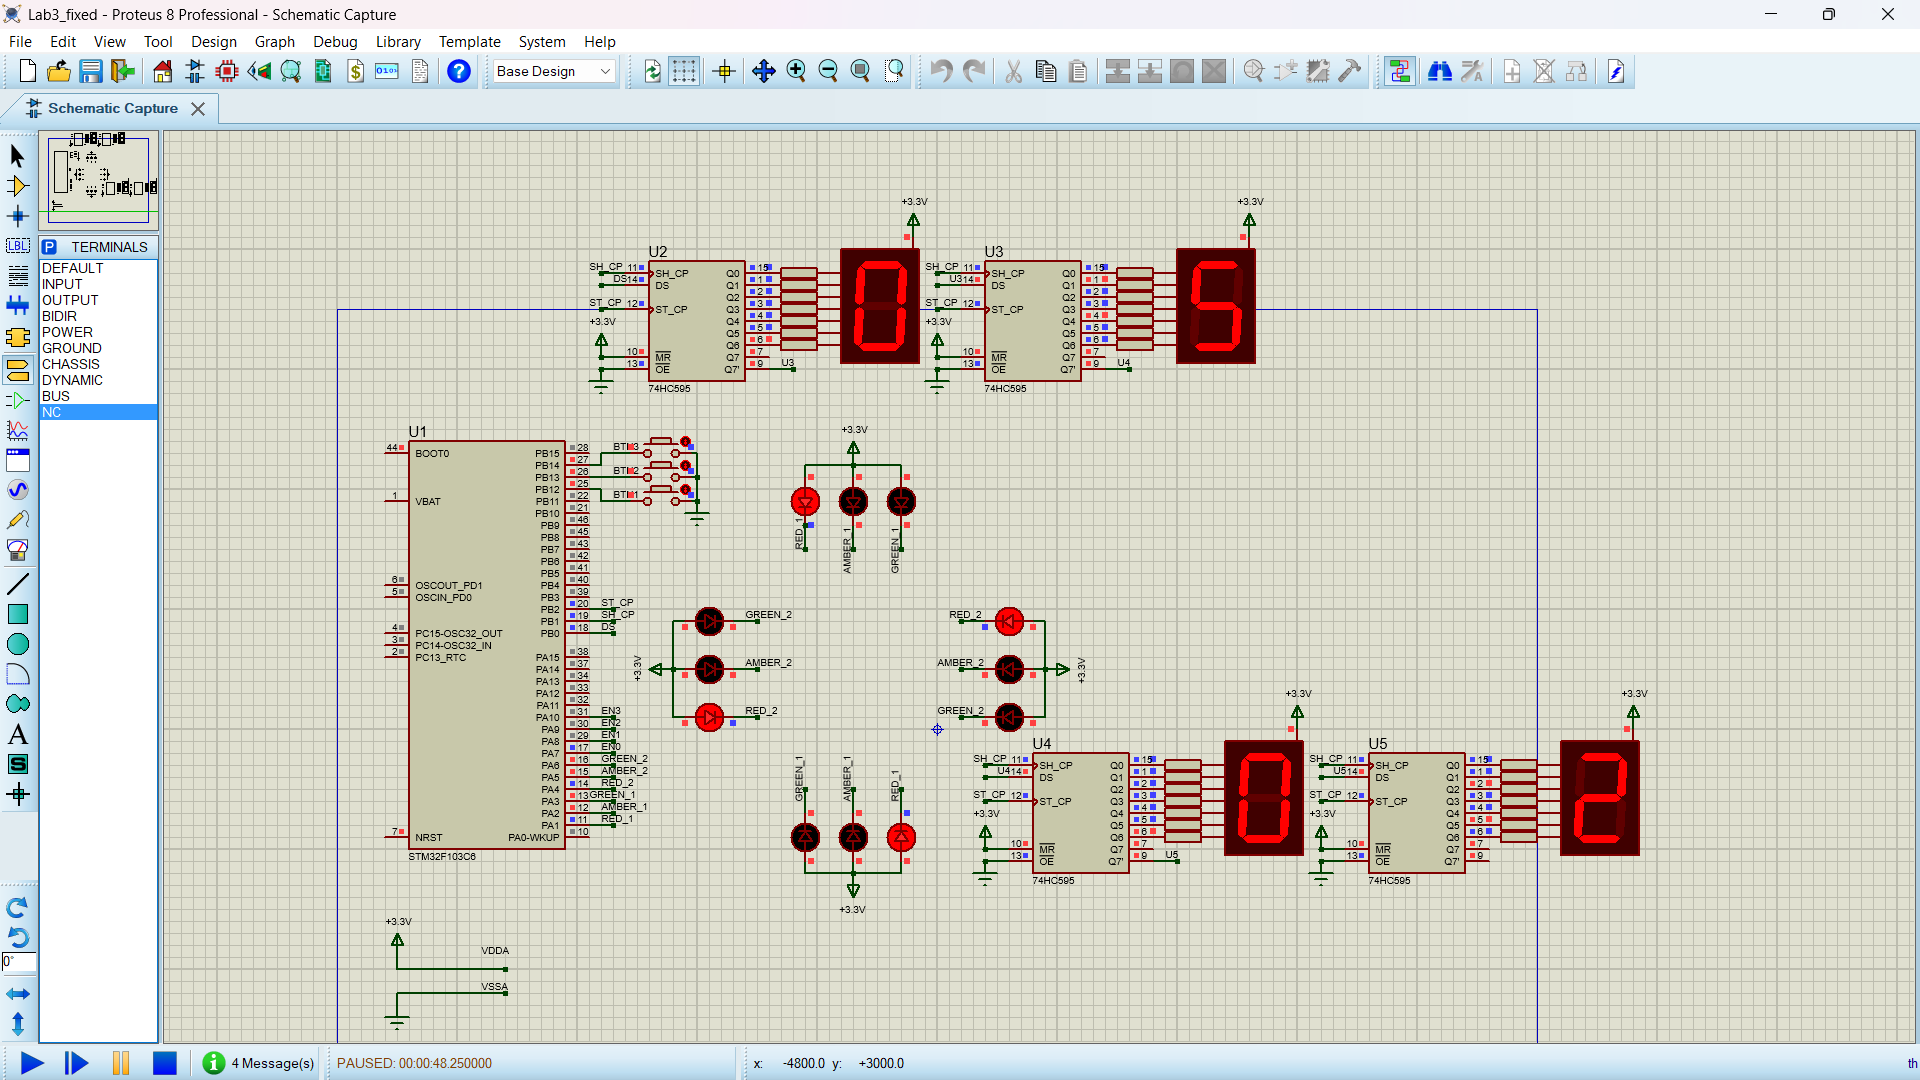
\includegraphics[width=\textwidth,height=0.65\textheight,keepaspectratio]{evidence_mode2.png}
    \caption{Mode 2: red duration 05 and mode indicator 02}
    \label{fig:evidence-mode2}
\end{figure}

\section{Exercise 8}

In mode 3, BTN2 increases the temporary amber duration by one. The value
wraps from 99 to 1. BTN3 copies the temporary value to the saved amber
duration. U2/U3 show the edited value and U4/U5 show mode 03.
The mode does not change when BTN3 is pressed.

\noindent\begin{minipage}{\linewidth}
\begin{lstlisting}[caption={Amber duration event handling excerpt -- Exercise 8}]
if (((events & 2U) != 0U) && (mode == 3U))
{
  temp_amber_duration = (temp_amber_duration >= 99U)
      ? 1U : (uint8_t)(temp_amber_duration + 1U);
  Display_UpdateBuffer();
}

if (((events & 4U) != 0U) && (mode == 3U))
{
  amber_duration = temp_amber_duration;
  Display_UpdateBuffer();
}
\end{lstlisting}
\end{minipage}

The simulation snapshot shows the amber adjustment mode with duration 02
and mode number 03. The four amber LEDs are captured in the on state.

\begin{figure}[H]
    \centering
    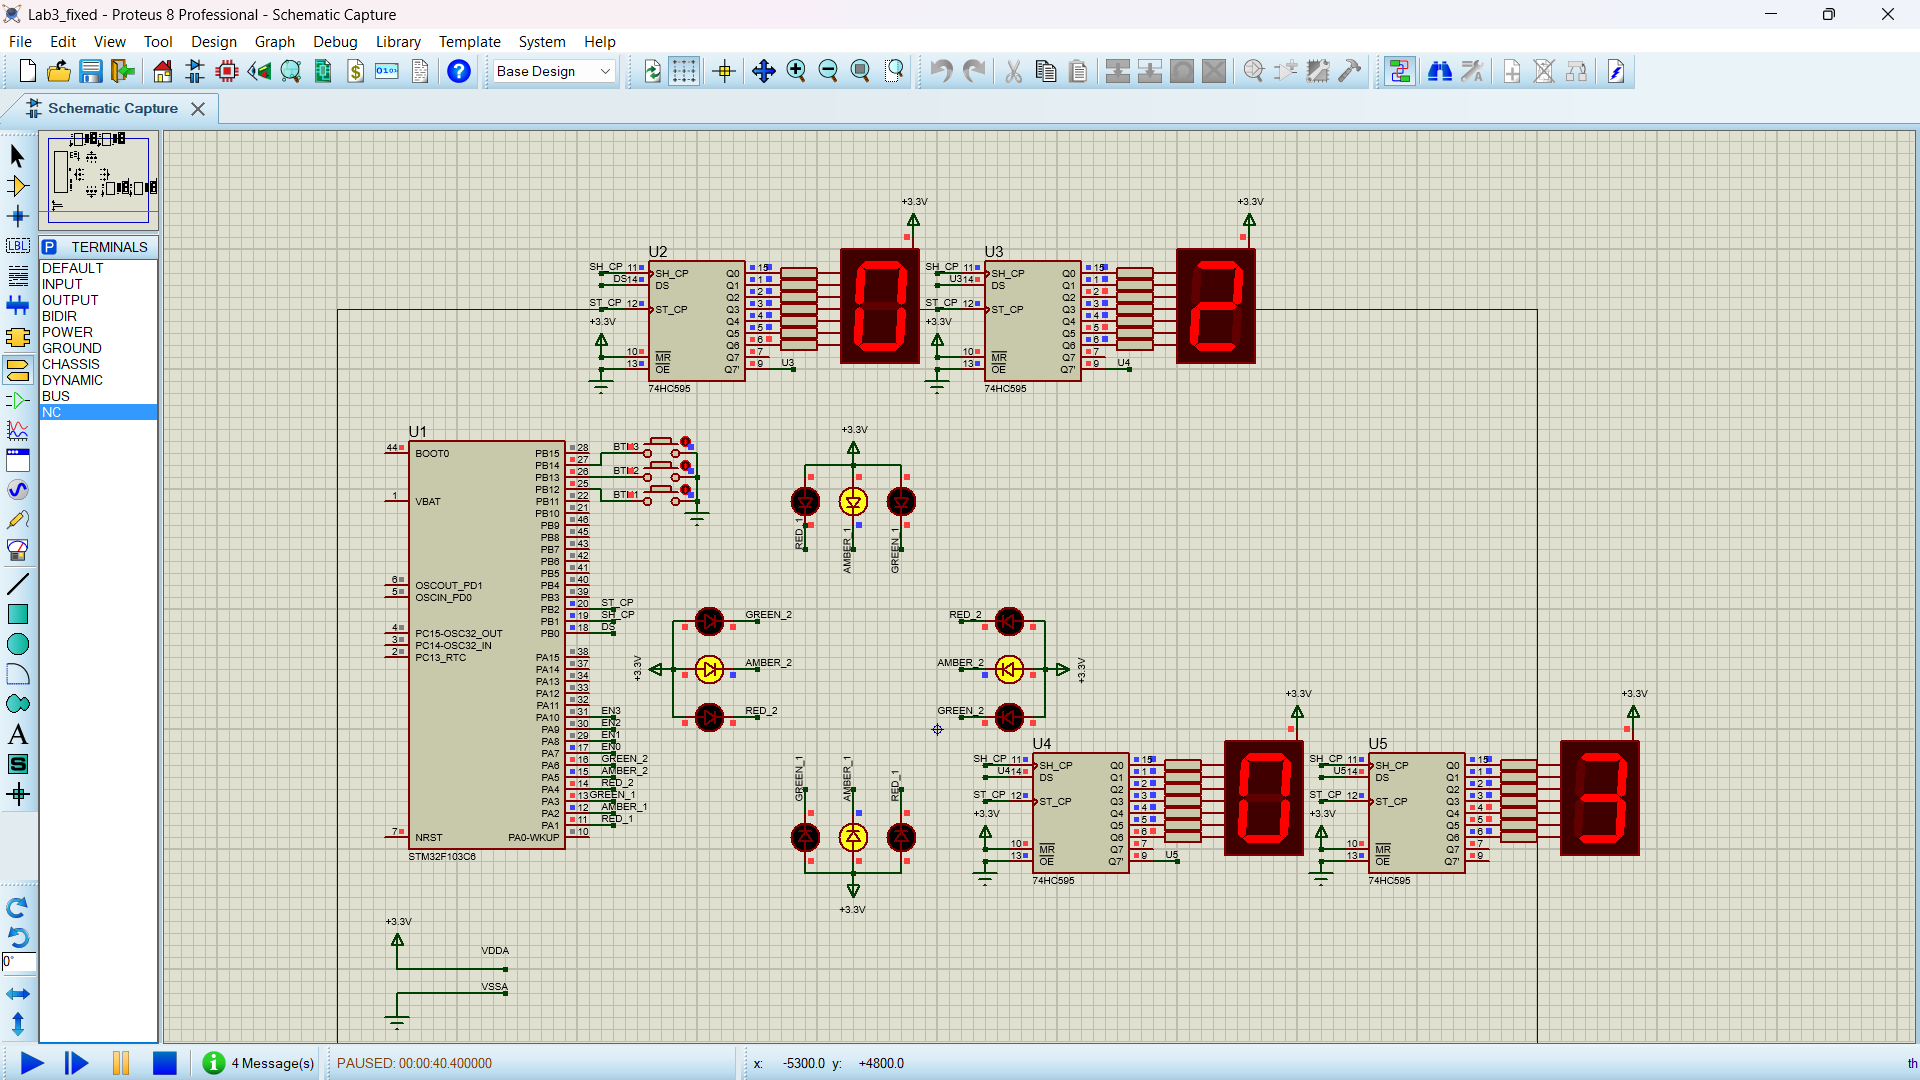
\includegraphics[width=\textwidth,height=0.65\textheight,keepaspectratio]{evidence_mode3.png}
    \caption{Mode 3: amber duration 02 and mode indicator 03}
    \label{fig:evidence-mode3}
\end{figure}

\section{Exercise 9}

In mode 4, BTN2 increases the temporary green duration by one. The value
wraps from 99 to 1. BTN3 copies the temporary value to the saved green
duration. U2/U3 show the edited value and U4/U5 show mode 04.
The mode does not change when BTN3 is pressed.

\noindent\begin{minipage}{\linewidth}
\begin{lstlisting}[caption={Green duration event handling excerpt -- Exercise 9}]
if (((events & 2U) != 0U) && (mode == 4U))
{
  temp_green_duration = (temp_green_duration >= 99U)
      ? 1U : (uint8_t)(temp_green_duration + 1U);
  Display_UpdateBuffer();
}

if (((events & 4U) != 0U) && (mode == 4U))
{
  green_duration = temp_green_duration;
  Display_UpdateBuffer();
}
\end{lstlisting}
\end{minipage}

The simulation snapshot shows the green adjustment mode with duration 03
and mode number 04. The four green LEDs are captured in the on state.

\begin{figure}[H]
    \centering
    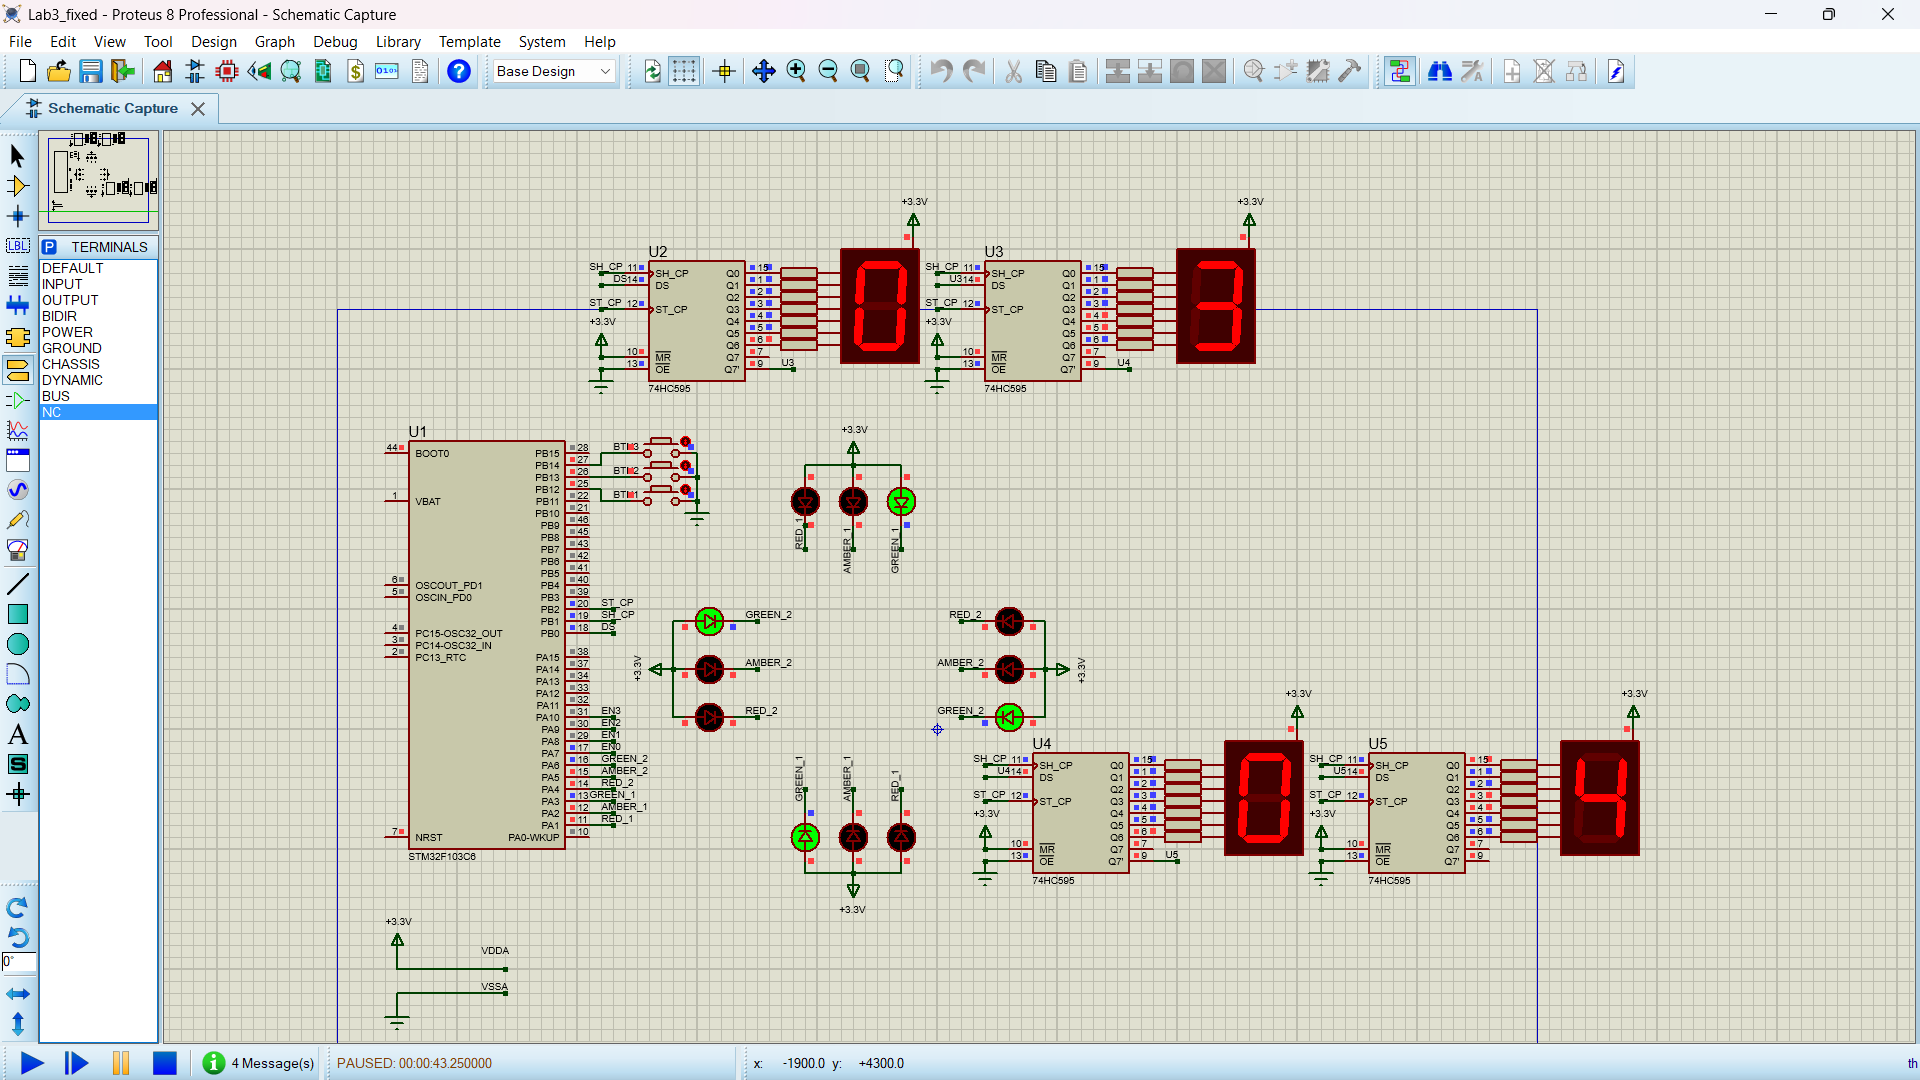
\includegraphics[width=\textwidth,height=0.65\textheight,keepaspectratio]{evidence_mode4.png}
    \caption{Mode 4: green duration 03 and mode indicator 04}
    \label{fig:evidence-mode4}
\end{figure}

\section{Exercise 10}

The normal-mode snapshot shows road 1 red with 04 seconds remaining and
road 2 green with 02 seconds remaining.

\begin{figure}[H]
    \centering
    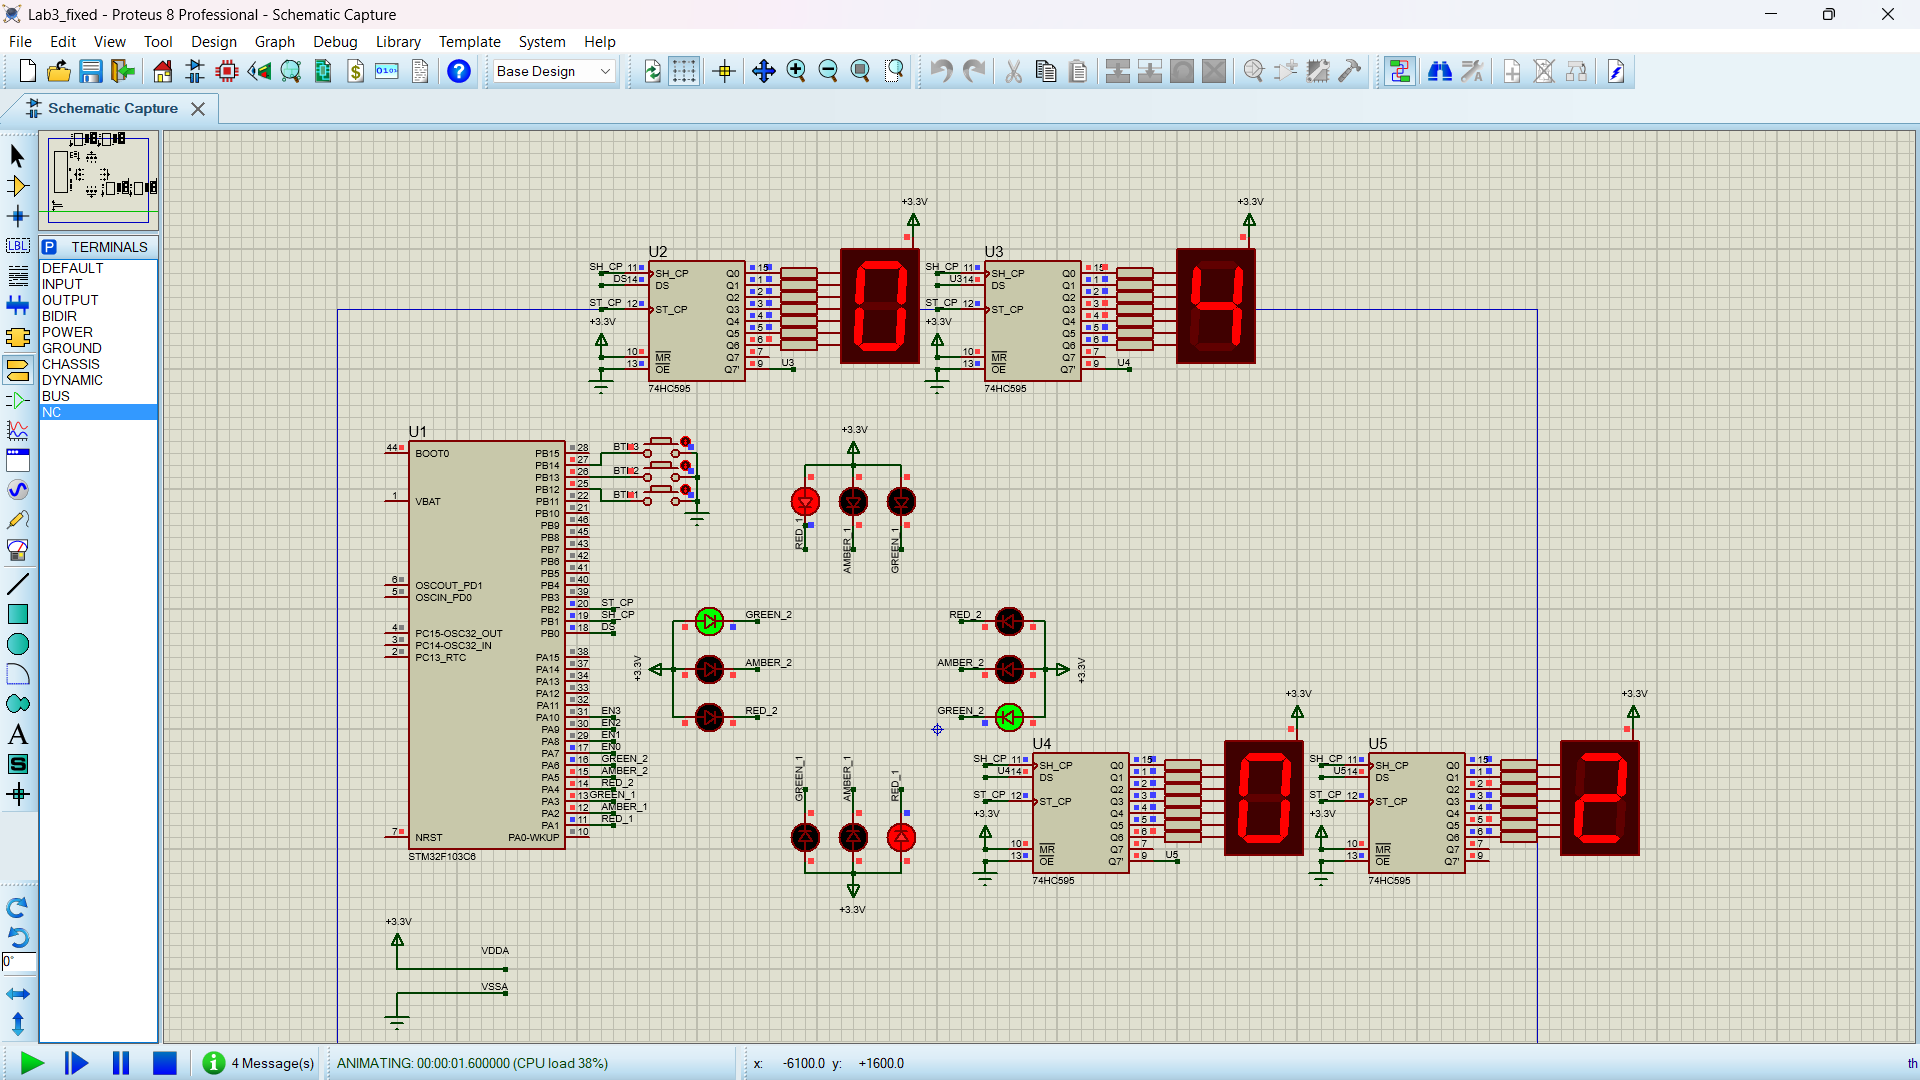
\includegraphics[width=\textwidth,height=0.65\textheight,keepaspectratio]{evidence_normal.png}
    \caption{Normal operation: road 1 countdown 04 and road 2 countdown 02}
    \label{fig:evidence-normal}
\end{figure}

The final project combines button debouncing, mode selection, duration editing,
traffic light sequencing, and static display output. The default durations are
5 s for red, 2 s for amber, and 3 s for green. Road 1 starts red while road 2
starts green. Each countdown is updated once per simulated second.

\begin{lstlisting}[caption={Normal traffic sequence -- Exercise 10}]
static void Traffic_InitNormal(void)
{
  road1_state = TRAFFIC_RED;
  road2_state = TRAFFIC_GREEN;
  road1_countdown = red_duration;
  road2_countdown = green_duration;
  Traffic_SetNormalLeds();
}

static void Traffic_Tick1s(void)
{
  if (road1_countdown > 1U)
  {
    road1_countdown--;
  }
  else
  {
    if (road1_state == TRAFFIC_RED)
    {
      road1_state = TRAFFIC_GREEN;
      road1_countdown = green_duration;
    }
    else if (road1_state == TRAFFIC_GREEN)
    {
      road1_state = TRAFFIC_AMBER;
      road1_countdown = amber_duration;
    }
    else
    {
      road1_state = TRAFFIC_RED;
      road1_countdown = red_duration;
    }
  }

  if (road2_countdown > 1U)
  {
    road2_countdown--;
  }
  else
  {
    if (road2_state == TRAFFIC_GREEN)
    {
      road2_state = TRAFFIC_AMBER;
      road2_countdown = amber_duration;
    }
    else if (road2_state == TRAFFIC_AMBER)
    {
      road2_state = TRAFFIC_RED;
      road2_countdown = red_duration;
    }
    else
    {
      road2_state = TRAFFIC_GREEN;
      road2_countdown = green_duration;
    }
  }

  Traffic_SetNormalLeds();
}
\end{lstlisting}

\noindent\begin{minipage}{\linewidth}
\begin{lstlisting}[caption={Integrated main function -- Exercise 10}]
int main(void)
{
  HAL_Init();
  SystemClock_Config();

  MX_GPIO_Init();
  MX_TIM2_Init();

  HAL_TIM_Base_Start_IT(&htim2);

  Buttons_Init();
  display_valid = 0U;
  traffic_1s_prev_ms = Timer_NowMs();
  blink_prev_ms = Timer_NowMs();
  blink_state = 1U;

  Traffic_InitNormal();
  Display_UpdateBuffer();

  while (1)
  {
    Input_Process();

    if (mode == 1U)
    {
      if (Timer_HasElapsed(&traffic_1s_prev_ms, 1000U))
      {
        Traffic_Tick1s();
        Display_UpdateBuffer();
      }
    }
    else
    {
      if (Timer_HasElapsed(&blink_prev_ms, BLINK_HALF_PERIOD_MS))
      {
        blink_state = (uint8_t)(!blink_state);
        Traffic_SetBlinkLeds();
      }
    }
    __WFI();
  }
}
\end{lstlisting}
\end{minipage}

Returning to normal mode restarts the sequence with the saved values. Durations
are stored in RAM and return to their defaults after reset. The implementation
allows each duration to be edited independently. For coordinated two-road
operation, the selected red duration must equal the green duration plus the
amber duration; this relationship is not enforced by the input code.

The firmware was built as \texttt{lab3\_74hc595.hex}. Host checks covered
10,000 display combinations, register order, 32 clock pulses per transfer,
active-low segment patterns, and suppression of repeated identical transfers.
Button checks covered mode changes, increasing a value, and saving it.
The final display was also confirmed working in Proteus after setting the
VCC/VDD supply to 3.3 V.

The demonstration video is available at
\href{https://drive.google.com/file/d/1mSy8i7v73HCMJG2kQaJ_mmHTSjQvnKNP/view?usp=sharing}{Lab 3 demonstration video (Google Drive)}.

\end{document}
